
\begin{figure}[hp]
% 
\begin{subfigure}[t]{.5\linewidth}
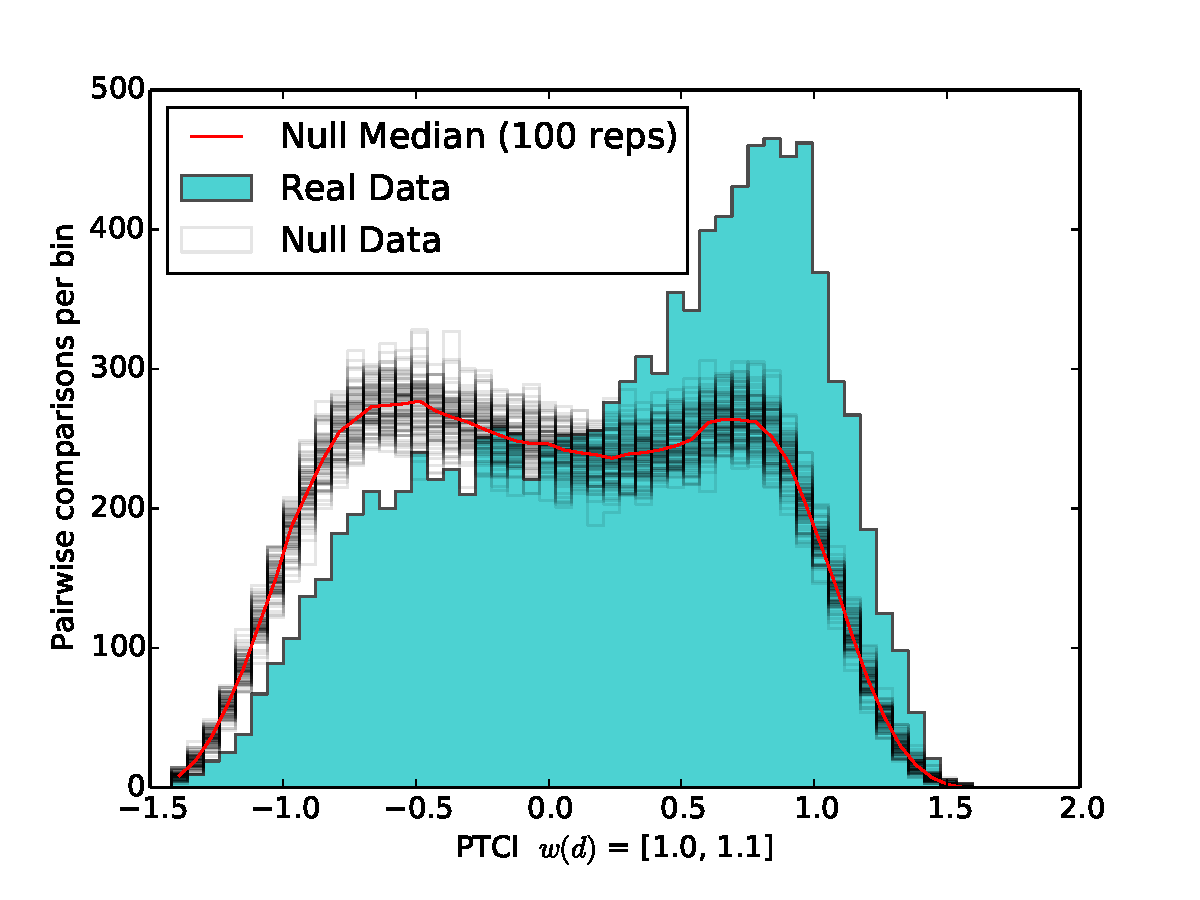
\includegraphics[width=\linewidth]{/home/gus/Dropbox/repos/git/uci-thesis-latex/figures/figs/ecr_team_ptci/pairwise_ptci_hist.pdf}
\caption{}
\label{fig:pairwise-ptci-hists-base}
\end{subfigure}%
\quad
\begin{subfigure}[t]{.5\linewidth}
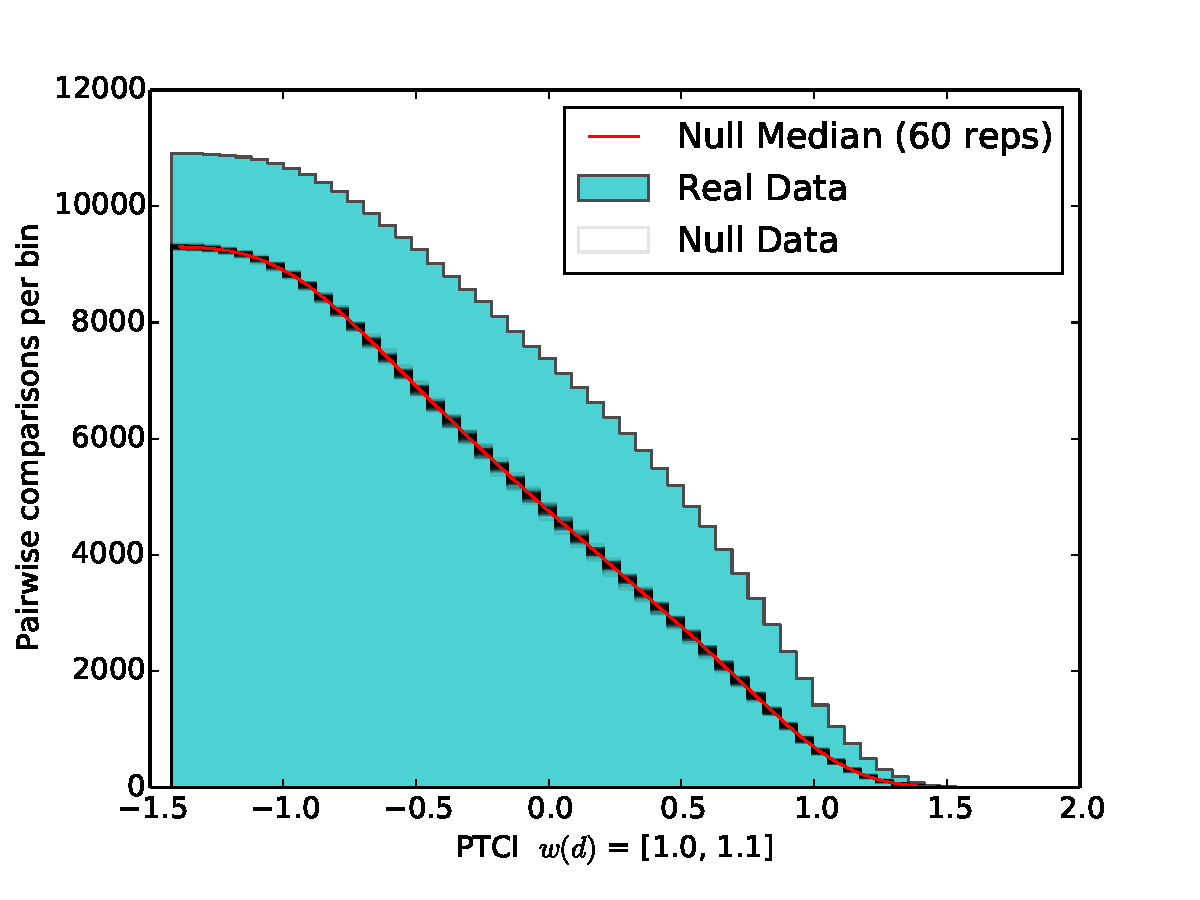
\includegraphics[width=\linewidth]{/home/gus/Dropbox/repos/git/uci-thesis-latex/figures/figs/ecr_team_ptci/pairwise_ptci_cum_hist.pdf}
\caption{}
\label{fig:pairwise-ptci-hists-rcum-hist}
\end{subfigure}
% 
\begin{subfigure}[t]{.5\linewidth}
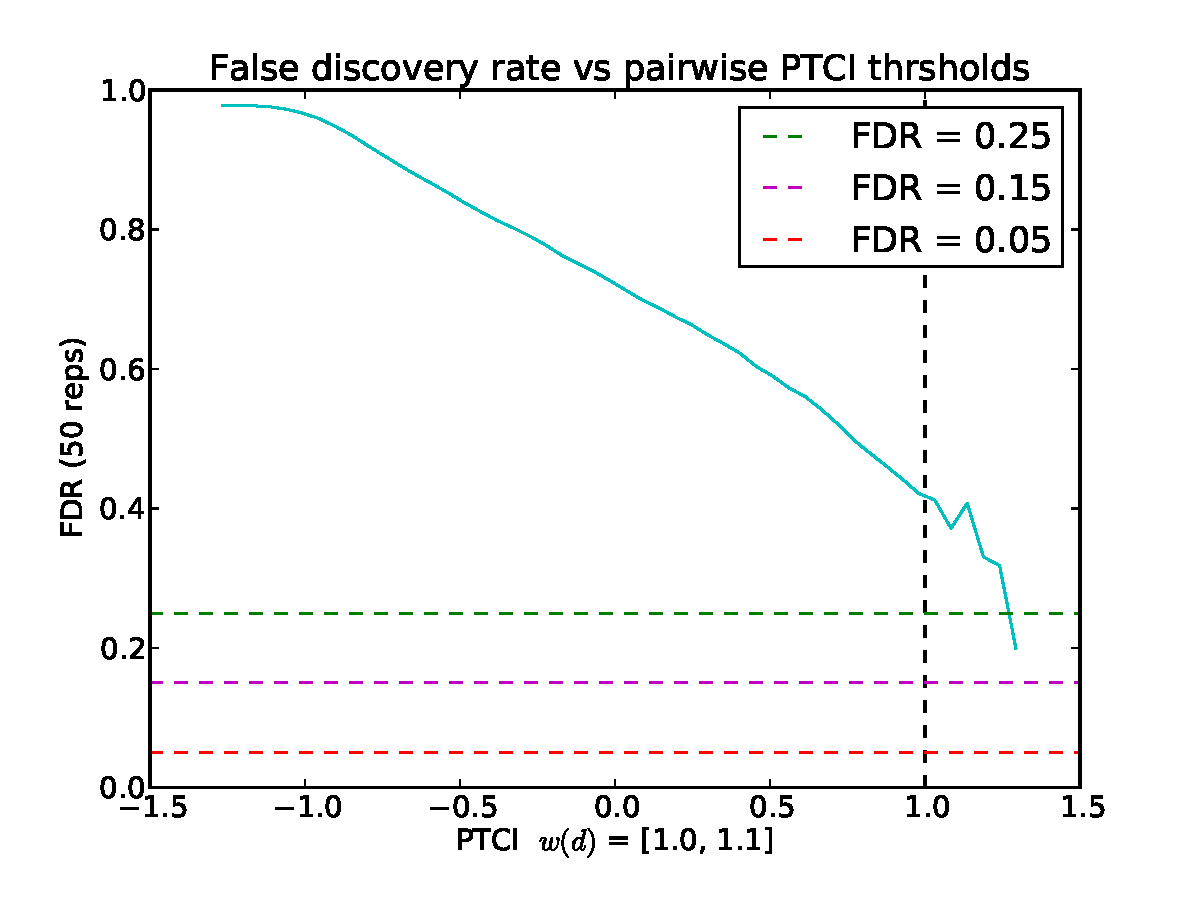
\includegraphics[width=\linewidth]{/home/gus/Dropbox/repos/git/uci-thesis-latex/figures/figs/ecr_team_ptci/pairwise_ptci_fdr.pdf}
\caption{}
\label{fig:pairwise-ptci-hists-fdr}
\end{subfigure}
% 
\caption[Pairwise PTCI results]{\sf \textbf{Pairwise PTCI results}:\\
\textbf{(A)} Histogram of pairwise PTCI results vs null distributions.
\textbf{(B)} Reverse Cumulative histogram of pairwise PTCI results vs null distributions.
\textbf{(C)} False discover rate vs PTCI threshold.}
\label{fig:pairwise-ptci-hists}
\end{figure}